\documentclass{memoir}

%%%%%%%%%%%%%%%%%%%%%%%%%%%%%%%%%%%%%%%%%
% Lachaise Assignment
% Structure Specification File
% Version 1.0 (26/6/2018)
%
% This template originates from:
% http://www.LaTeXTemplates.com
%
% Authors:
% Marion Lachaise & François Févotte
% Vel (vel@LaTeXTemplates.com)
%
% License:
% CC BY-NC-SA 3.0 (http://creativecommons.org/licenses/by-nc-sa/3.0/)
% 
%%%%%%%%%%%%%%%%%%%%%%%%%%%%%%%%%%%%%%%%%

%----------------------------------------------------------------------------------------
%	PACKAGES AND OTHER DOCUMENT CONFIGURATIONS
%----------------------------------------------------------------------------------------

\usepackage{amsmath,amsfonts,stmaryrd,amssymb} % Math packages

\usepackage{enumerate} % Custom item numbers for enumerations

\usepackage[ruled]{algorithm2e} % Algorithms

\usepackage[framemethod=tikz]{mdframed} % Allows defining custom boxed/framed environments

\usepackage{listings} % File listings, with syntax highlighting
\lstset{
	basicstyle=\ttfamily, % Typeset listings in monospace font
}

%----------------------------------------------------------------------------------------
%	DOCUMENT MARGINS
%----------------------------------------------------------------------------------------

\usepackage{geometry} % Required for adjusting page dimensions and margins

\geometry{
	paper=a4paper, % Paper size, change to letterpaper for US letter size
	top=2.5cm, % Top margin
	bottom=3cm, % Bottom margin
	left=2.5cm, % Left margin
	right=2.5cm, % Right margin
	headheight=14pt, % Header height
	footskip=1.5cm, % Space from the bottom margin to the baseline of the footer
	headsep=1.2cm, % Space from the top margin to the baseline of the header
	%showframe, % Uncomment to show how the type block is set on the page
}

%----------------------------------------------------------------------------------------
%	FONTS
%----------------------------------------------------------------------------------------

\usepackage[utf8]{inputenc} % Required for inputting international characters
\usepackage[T1]{fontenc} % Output font encoding for international characters

\usepackage{XCharter} % Use the XCharter fonts

%----------------------------------------------------------------------------------------
%	COMMAND LINE ENVIRONMENT
%----------------------------------------------------------------------------------------

% Usage:
% \begin{commandline}
%	\begin{verbatim}
%		$ ls
%		
%		Applications	Desktop	...
%	\end{verbatim}
% \end{commandline}

\mdfdefinestyle{commandline}{
	leftmargin=10pt,
	rightmargin=10pt,
	innerleftmargin=15pt,
	middlelinecolor=black!50!white,
	middlelinewidth=2pt,
	frametitlerule=false,
	backgroundcolor=black!5!white,
	frametitle={Command Line},
	frametitlefont={\normalfont\sffamily\color{white}\hspace{-1em}},
	frametitlebackgroundcolor=black!50!white,
	nobreak,
}

% Define a custom environment for command-line snapshots
\newenvironment{commandline}{
	\medskip
	\begin{mdframed}[style=commandline]
}{
	\end{mdframed}
	\medskip
}

%----------------------------------------------------------------------------------------
%	FILE CONTENTS ENVIRONMENT
%----------------------------------------------------------------------------------------

% Usage:
% \begin{file}[optional filename, defaults to "File"]
%	File contents, for example, with a listings environment
% \end{file}

\mdfdefinestyle{file}{
	innertopmargin=1.6\baselineskip,
	innerbottommargin=0.8\baselineskip,
	topline=false, bottomline=false,
	leftline=false, rightline=false,
	leftmargin=2cm,
	rightmargin=2cm,
	singleextra={%
		\draw[fill=black!10!white](P)++(0,-1.2em)rectangle(P-|O);
		\node[anchor=north west]
		at(P-|O){\ttfamily\mdfilename};
		%
		\def\l{3em}
		\draw(O-|P)++(-\l,0)--++(\l,\l)--(P)--(P-|O)--(O)--cycle;
		\draw(O-|P)++(-\l,0)--++(0,\l)--++(\l,0);
	},
	nobreak,
}

% Define a custom environment for file contents
\newenvironment{file}[1][File]{ % Set the default filename to "File"
	\medskip
	\newcommand{\mdfilename}{#1}
	\begin{mdframed}[style=file]
}{
	\end{mdframed}
	\medskip
}

%----------------------------------------------------------------------------------------
%	NUMBERED QUESTIONS ENVIRONMENT
%----------------------------------------------------------------------------------------

% Usage:
% \begin{question}[optional title]
%	Question contents
% \end{question}

\mdfdefinestyle{question}{
	innertopmargin=1.2\baselineskip,
	innerbottommargin=0.8\baselineskip,
	roundcorner=5pt,
	nobreak,
	singleextra={%
		\draw(P-|O)node[xshift=1em,anchor=west,fill=white,draw,rounded corners=5pt]{%
		Question \theQuestion\questionTitle};
	},
}

\newcounter{Question} % Stores the current question number that gets iterated with each new question

% Define a custom environment for numbered questions
\newenvironment{question}[1][\unskip]{
	\bigskip
	\stepcounter{Question}
	\newcommand{\questionTitle}{~#1}
	\begin{mdframed}[style=question]
}{
	\end{mdframed}
	\medskip
}

%----------------------------------------------------------------------------------------
%	WARNING TEXT ENVIRONMENT
%----------------------------------------------------------------------------------------

% Usage:
% \begin{warn}[optional title, defaults to "Warning:"]
%	Contents
% \end{warn}

\mdfdefinestyle{warning}{
	topline=false, bottomline=false,
	leftline=false, rightline=false,
	nobreak,
	singleextra={%
		\draw(P-|O)++(-0.5em,0)node(tmp1){};
		\draw(P-|O)++(0.5em,0)node(tmp2){};
		\fill[black,rotate around={45:(P-|O)}](tmp1)rectangle(tmp2);
		\node at(P-|O){\color{white}\scriptsize\bf !};
		\draw[very thick](P-|O)++(0,-1em)--(O);%--(O-|P);
	}
}

% Define a custom environment for warning text
\newenvironment{warn}[1][Warning:]{ % Set the default warning to "Warning:"
	\medskip
	\begin{mdframed}[style=warning]
		\noindent{\textbf{#1}}
}{
	\end{mdframed}
}

%----------------------------------------------------------------------------------------
%	INFORMATION ENVIRONMENT
%----------------------------------------------------------------------------------------

% Usage:
% \begin{info}[optional title, defaults to "Info:"]
% 	contents
% 	\end{info}

\mdfdefinestyle{info}{%
	topline=false, bottomline=false,
	leftline=false, rightline=false,
	nobreak,
	singleextra={%
		\fill[black](P-|O)circle[radius=0.4em];
		\node at(P-|O){\color{white}\scriptsize\bf i};
		\draw[very thick](P-|O)++(0,-0.8em)--(O);%--(O-|P);
	}
}

% Define a custom environment for information
\newenvironment{info}[1][Info:]{ % Set the default title to "Info:"
	\medskip
	\begin{mdframed}[style=info]
		\noindent{\textbf{#1}}
}{
	\end{mdframed}
}
 % Include the file specifying the document structure and custom commands

\usepackage{enumitem}
\usepackage{fancyhdr}
\usepackage{algorithm}
\usepackage{algorithmic}
\usepackage[utf8]{inputenc}
\usepackage[english]{babel}
\usepackage{biblatex}
% \usepackage{algorithmicx}
\usepackage{float}
\pagestyle{fancy}
\fancyhf{}
\rhead{IIIT Bangalore}
\lhead{CS825 - Graph Theory}
\cfoot{\thepage}

\title{\fontfamily{ptm}\selectfont{\textbf{BLOCK GRAPHS}}} % Title of the assignment

\author{
        \textbf{Bishwajeet Kumar Sharma}\\ 
        \text{MT2020169}\\
        bishwajeet.sharma@iiitb.ac.in
        \and
        \textbf{Milan Gupta}\\
        \text{MT2020120}\\
        milan.gupta@iiitb.ac.in
        \and
        \textbf{Himanshu Singh}\\
        \text{MT2020143}\\
        himanshu.singh@iiitb.ac.in
} 
\date{IIIT Bangalore}


\begin{document}

\maketitle % Print the title


\section*{DEFINITION}
\subsection{Block}
\\A graph is called a block if it has more
than one vertex, and is 2-connected. A block of a graph $G$ is a maximal subgraph of $G$ which is itself a block. 
\subsection{Block Graph}
\\The block graph $B(G)$ of a given graph G is the graph whose vertex set is the set of blocks {$B_1$,$B_2$,..,$B_i$} of G and whose edges are determined by taking two vertices $B_1$ and $B_2$ as adjacent if and only if they contain a cut vertex of original graph $G$ in common.
\\
\\A graph is called a block graph if it is the block graph of some graph $G$. 
\begin{figure}[htp]
    \centering
    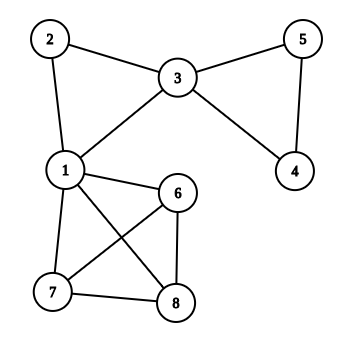
\includegraphics[width=5cm]{graph.png}
    \caption{A block graph}
    \label{fig:1}
\end{figure}

\subsection{Equivalent definitions}
A graph is a block graph if for every four vertices u,v,w,x in the same connected component d(u,v)+ d(w,x) <= max( d(u,w)+ d(v,x), d(u,x)+ d(v,w) ).
\\
\\
A graph is a block graph if for every four vertices u,v,w,x in the same connected component the larger two of the distance sums
d(u,v)+ d(w,x)
d(u,w)+ d(v,x)
d(u,x)+ d(v,w)
are equal.
\section*{Construction of a block graph}
\begin{itemize}
    \item We consider a simple, undirected graph G(V,E), where V is a non-empty set of vertices and E is a non-empty set of edges.
    \item If the graph is not having a cut-vertex, then it is at least 2-connected and is maximal, hence it is a block graph.
    \item If the graph is having one or more cut vertices, then we remove a cut vertex and consider all the components of the graph.
    \item We then add the removed cut vertex to each component by connecting it with the vertices it was adjacent to in the original graph.
    \item If any of the components are still 1-connected then we repeat the same steps until no component is one connected and the whole graph is now divided into blocks.
    \item We consider the set of each of these blocks , say , $F={B_1,B_2,...,B_n}$ as the set of vertices and two blocks $B_1$ and $B_2$ are connected if they share a common cut-vertex.
    \item Thus, the intersection graph of the blocks of set $F$ is the block graph, denoted by $B(G)$.
    
\end{itemize}

\section*{CHARACTERISTICS} % Numbered section

A graph invariant is a number related to a graph which is structurally invariant, that is to say it is fixed under graph automorphisms These invariants are also called topological index. \\The Wiener index, denoted by \textbf{W} is defined as the sum of all distances between the vertices of a graph. It is a distance based graph invariant.
\begin{equation}
    W(G)=\sum_{{u,v}\in{V(G)}}d(u,v)
\end{equation}
\\Another topological index is known as Szeged index, which is a vertex multiplicative type index.
\begin{equation}
    Sz(G)=\sum_{{u,v}\in{E(G)}}n_e(u) n_e(v)
\end{equation}
where $n_e(u)$ is the cardinality of the set $N_e(u)$ (set of all vertices v which are at a distance of unity from u).
\\
\begin{itemize}
    \item For a graph G, if $W(G)=Sz(G)$, then $G$ is a block graph.
    \item The intersection of any two distinct blocks of a graph consists of at most one point. And, this common point is a cut-vertex of the original graph.
    \item Block graphs can be formed by the intersection of blocks of any arbitrary undirected graph, where blocks are maximal biconnected subgraphs of a given graph.
    \item For every four vertices u, v, w, and x, the largest two of the three distances d(u,v) + d(w,x), d(u,w) + d(v,x), and d(u,x) + d(w,v) are always equal.
    \item Block graphs are a sub class of Chordal graphs. Hence, they are perfect graphs also.
    \item Block graphs do not have the diamond graph( $K_4$ - $e$ )as an induced subgraph. Hence, they are also called diamond free chordal graphs.
    \item Since each block in a forest is either K\textsubscript{1} or K\textsubscript{2}, Block graphs is a superset of the class of forests. 
    \item Block graphs are proper subclass of triangulated graphs, which are the graphs that does not contain simple cycles of size four or more as an induced subgraph.
\end{itemize}
\section*{Theorems on Block-graphs}
\subsection{Theorem 1: If H is a block-graph, then every block of H is complete. }
\textbf{Proof:}Suppose there exists a simple graph $G$, and a block graph $H$, such that $H=B(G)$.\ By contradiction, we assume that there exists a block of $H$, say , $H_1$, such that two vertices $u_1$ and $u_2$ of $H_1$ are not adjacent. Since, $H_1$ is a block and without violating the definition of a block we can assume that these two vertices lie on a cycle which must be of length greater than 4. Since, vertices $u_1$ and $u_2$ must be corresponding to blocks $B_1$ and $B_2$ of the original graph $G$, and, $u_1$ and $u_2$ not being adjacent means that blocks $B_1$ and $B_2$ are not sharing any cut-vertex in the original graph, which means $B_1$ and $B_2$ are not maximal 2-connected subgraphs. This is a contradiction and therefore every block of a block graph is complete.

\subsection{Theorem 2: If every block of H is complete, then H is a block-graph.}
\subsubsection{Proof by construction:}\\
\begin{itemize}
    \item We consider a graph $H$, whose every block is complete.
    \item We construct a block graph $B(H)$ of $H$.
    \item After this, we construct a new graph $G$ from $B(H)$ by adding edges to each vertex $H_i$ of $B(H)$ corresponding to the number of non cut-vertices in the block $B_i$ corresponding to the vertex $H_i$.
    \item Now, if we construct the block graph of $G$, $B(G)$, then $B(G)$ will be isomorphic to $H$.
    \item Hence, $H$ is isomorphic to a block graph.
    \item Hence, $H$ is a block graph.
 \end{itemize}
 Therefore, from the above two theorems, we can state that a graph is a block- graph if and only if all its blocks are complete. \begin{figure}[htp]
    \centering
    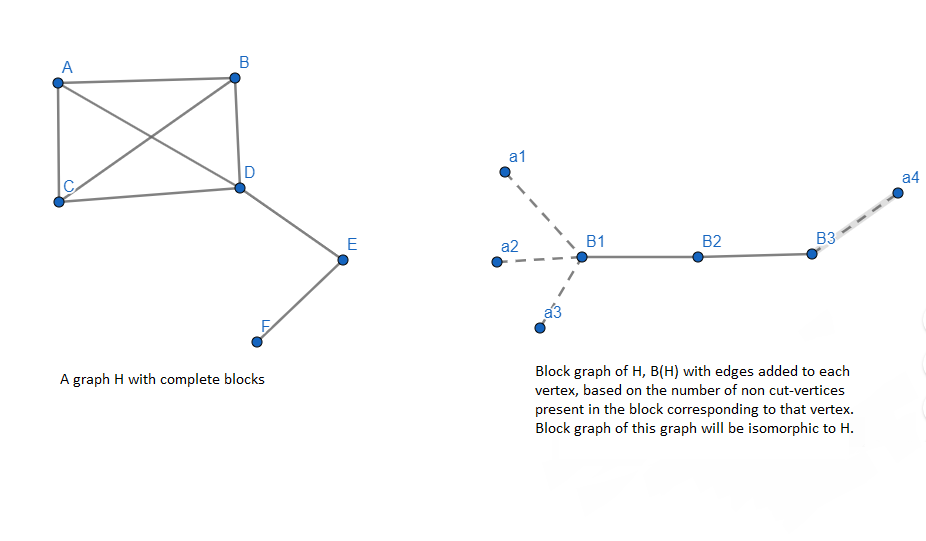
\includegraphics[width=15cm,scale=1.5]{theorem2.png}
    \caption{Pictorial representation of the construction}
    \label{fig:1}
\end{figure}
\\
\\
Since, a diamond graph is not a complete block, hence we cannot have a diamond graph as an induced subgraph of a block graph.
% }
\section*{Recognization of block graphs}

The blocks in a block graph are complete and it's well known that a graph $G$ of order $n$ is complete if and only if $G$ has $n(n-1)/2$ edges. Thus the completeness of a graph can be determined in linear time. Hence, given blocks $B$ of a graph $G$, we just need to check whether they have $n(n-1)/2$ edges or not. This can be done in linear time.

John Hopcroft and Robert Tarjan (1973) have proved that the biconnected components in a connected undirected graph and the blocks of a connected graph can be found in linear time and their algorithm was based on depth first search.
Therefore, we can say that there is a linear time algorithm which recognizes the class of block graphs, given the different blocks in the graph.
% \vspace{5mm}
\section*{Vertex Cover}

Problem: Given a graph $G(V, E)$, the vertex cover of $G$ is a set of vertices, V\textsubscript{c}, such that every edge in $G$ has at least one of the vertex in V\textsubscript{c} as an endpoint. This means that the set V\textsubscript{c} covers every edge of $G$.

Similarly, finding the smallest size of V\textsubscript{c} in $G$ is referred to as the minimum vertex cover problem and is denoted by \begin{math}
    \tau (G). \end{math}

The vertex cover problem is an NP-complete problem, it was one of Karp's 21 NP-complete problems and is often used in computational complexity theory as a starting point for NP-hardness proofs.There are approximate polynomial-time algorithms to solve the problem though.

Following is the simple approximate algorithm for the vertex cover:

\begin{center}
\caption{\texttt{APPROXIMATION-VERTEX-COVER$(G = (V, E))$}}
		\begin{algorithmic}[H]
            \SetAlgoLined
            \texttt{C = empty set\\
            E' = E\\
             \While{E' $\neq$ E}{
                let (u, v) be an arbitrary edge of E'\\
                add u and v to C\\
                remove from E' all edges incident to u and v
             }
             \textbf{return} C
            %  \eIf{condition}{
            %   instructions1\;
            %   instructions2\;
            %   }{
            %   instructions3\;
            %   }
             }
            %  \caption{\texttt{APPROXIMATION-VERTEX-COVER$(G = (V, E))$}}
        \end{algorithmic}
\end{center}

There is no bounded algorithm known for the vertex cover problem of block graphs
% \vspace{5mm}
\section*{Independent Set}

Given a graph $G=(V, E)$, a subset $S$ of vertices $V$, is an independent set if there exists no edge between the vertices in $S$. The maximum independent set is the set having highest number of vertices i.e a set of largest possible size for $G$, which will result in the addition of an edge between the vertices in $S$ if any new vertex is added. This size is called the maximum independence number of $G$ and is denoted by \begin{math} \alpha (G) \end{math}.

Before stating the computational complexity of finding
the independent set of block graphs, we first take a look at a few properties of block graphs and then from these properties we will infer the time complexity of independent set problem:
\begin{itemize}[noitemsep]
  \item Block graph is acyclic.
  \item Block graph is connected.
  \item From the above two, block graph is a tree.
\end{itemize}

For trees, we know there exists a linear time algorithm for finding the independent set, and since a block graph is always a tree, it can be inferred that there also exists a linear time algorithm for finding the independent set of a block graph.
\\

\section*{Coloring Problem}

The coloring problem in graphs refers to the assignment of colors to the vertices of the graph so that no two adjacent vertices have the same color. The chromatic number of a graph G is the minimum number of colors required in a proper coloring; it is denoted by \begin{math} \chi (G). \end{math}
\\ Block graphs are a sub class of chordal graphs and chordal graphs are perfect graphs. Hence, the chromatic number of a block graph is equal to its maximum clique number and since we know that a chordal graph has also a Perfect Elimination Ordering, therefore we can obtain an optimal coloring by applying a greedy coloring algorithm to the vertices in reverse of the perfect elimination ordering.
\\
\\An algorithm by Tarjan and Yannakakis finds a perfect elimination ordering in linear time. This algorithm is called maximum cardinality search(MCS).The algorithm assigns an integer weight, w(v), for each vertex v  which is the number of adjacent vertices whose weight is positive. All weights are set to zero initially.
\begin{center}
    \begin{algorithmic}
                \SetAlgoLined
                \texttt{let Q = V be the set of vertices\\
                let PEO = [] be the perfect elimination order (initially empty)\\
                \For{all vertices x in Q}{
                weight(x)=0\\
                }
                \While{Q is not empty}{
                let x in Q be a vertex of maximum weight\\
                remove x from Q and append it to PEO\\
                \For{vertices z in Q \cap  Adj(x)}{
                weight(z) = weight(z) + 1\\}
                }
                }
    \end{algorithmic}
\end{center}

\\This algorithm can be implemented in O((n+m)lg n) using priority queue, where $n$=number of vertices and $m$=number of edges.
\\The claim is that this yields an optimal coloring. To prove this we have to show that the chromatic number $\chi(G)$ coincides with the clique number w(G).
\\The greedy algorithm chooses the smallest number not used among the predecessors to color the next vertex,  so the minimum number of colors $\chi(G)$ is at most $\max_i\{indeg(v_i)\}+1$, where i=1 to n.
\\Let $v_j$ be the vertex of maximum $indeg: \chi(G) \le indeg(v_j)+1$. Since we have a perfect elimination ordering( block graphs belong to the family of chordal graphs), $v_j$ is simplicial, and $v_j$ together with its predecessors forms a clique. So $w(G) \ge indeg(v_j)+1$. But we know that $\chi(G) \ge w(G)$. This implies that $\chi(G)=w(G)=indeg(v_j)+1$.

\section*{Dominating Set problem}
Let $G=(V,E)$ be an unweighted graph, $S \subseteq V$ is called dominating set in $G$ if for every vertex u not in $S$ is adjacent to atleast one vertex in $S$. A dominating set S is a minimal dominating set if no proper subset $S' \subseteq S$ is a dominating set. The domination number \begin{math} \gamma (G) \end{math} of a graph $G$ equals the minimum cardinality of a set in the minimal dominating set.\\
% \vspace{5mm}

Dominating set and Independent set are somewhere same like if an independent set is a maximal independent set then it is also a minimal dominant set.\\
% \vspace{5mm}

Also, finding a minimum dominating set is computationally hard and there is no polynomial time algorithm to compute this. The brute force approach could be to check all $n \choose k$ subsets $\subseteq V$ of size k and traverse k from 1 to n in steps till the minimum size dominating set is found. Though the problem is NP-complete, there are some efficient approximation algorithms there for some graph classes.\\

Zhuguo Mo, a scholar in 1988, presented a linear time algorithm for finding a minimum dominating set of radius r in an (unweighted) block-complete graph. The algorithm finds a minimum dominating set of radius r, U, in an arbitrary connected block-complete graph G. The process is carried out through a search on the blocks of G, starting from the end-blocks and moving toward the "middle. " During this search, the vertices of the
desired dominating set of radius r are located in an "optimal fashion" until
all vertices in the graph are dominated by vertices In U within
distance r. To do this, a copy G' of the original graph as an auxiliary graph is used on which the algorithm is carried out, and two variables C(v) and R(v)  are attached to each vertex v of G'. C(v) is a boolean variable which has value TRUE if v Is already dominated (within distance r) by some vertex in U and has value FALSE otherwise. If B is an end-block of the auxiliary graph G' and V\textsubscript{C} is the cut-vertex of B in G', then the variables C(V\textsubscript{C}) and R(V\textsubscript{C}) are updated and all
vertices In V(B) $-$ V\textsubscript{C} (including incident edges) from G' are removed. As a result, a new block may become an end-block of G', and the process is repeated until the graph G' becomes a complete graph. Then an
appropriate set of vertices is added to U if necessary.

The variable R(v) has the following Interpretation (based on C(v)):
\begin{itemize}[noitemsep]
    \item Case 1: If the vertex v is already dominated by one of the vertices in U which have been located so far, then R(v) is the distance between v and the nearest located vertex in U.
    \item Case 2: If the vertex Is not yet dominated, then let S(v) be
    the set of all the vertices of the original graph G which are not
    yet dominated, and for which v is the nearest vertex in the auxiliary graph G'. Notice that v Is the only vertex In S(v) which belongs to G'; In fact, S(v) is the set consisting of the vertex v and all those vertices which have already been removed from G' and are to be dominated by the same vertex of the dominating set of radius r as v.
\end{itemize}
The time complexity of this proposed algorithm is O(|E|+|V|) which is linear.

\vspace{5mm}

A set of vertices D is a total dominating set if
every vertex in V is adjacent to a vertex in D. The total domination problem is to determine the total domination number \begin{math} \gamma\textsubscript{t} (G) \end{math} which is the minimum cardinality of a total dominating set for a graph G. Total domination problem is also NP-complete for some graph classes like bipartite graphs, split graphs but polynomial time algorithm do exist for interval graphs, permutation graphs, trees, etc. And there exist an O(|E|+|V|) time algorithm presented by Gerard J. Chang in his paper in 1989 for the total domination problem in block graphs.

% 
%  \begin{center}
%  \caption{\texttt{Minimum Dominating Set of radius r for a connected block-complete graph $(G = (V, E))$}}
% 		\begin{algorithmic}
%             \SetAlgoLined
%             \texttt{G' <- G; U <- \emptyset} \\
%             % \texttt{
%             \For {each vertex v in G'}{
%                 C(v) <- FALSE; \\
%                 R(v) <- 0;
%                 }
%                 % }
            
%              \While{G' is not complete}{
%                 Find an end-block B In G' \\
%                 Let Vc be the cut-vertex of B In G' \\
%                 define  min{R(v)|v \in \emptyset }= r+ 1 \\
%                     and max{R(v)|v \in \emptyset }=0 \\
                    
%                 Rt <- min {(R(v)|v \in V(B) and C(v) = TRUE} \\
%                 Rf <- max {(R(v)|v \in V(B) and C(v) = FALSE} \\
%                 R' <- min {(R(v)|v(\neq v_c) \in V(B) and C(v) = TRUE} \\
%                 R'' <- max {(R(v)|v(\neq v_c) \in V(B) and C(v) = FALSE} \\
%                  Update C(v_c) and R(v_c) \\
                
%                 \eIf{C(v_c)}{
                
%                     \eIf{Rt + Rf + 1 \leq r}{
%                       R(v_c) <- min {R' + 1, R(v_c)} \\
%                         }{
%                          C(v_c) <- FALSE; R(v_c) <-  R" + 1 \\
%                          }
%                     }{
                
%                   \eIf{Rt + Rf +1 \leq r}{
%                       C(v_c) <- TRUE; R(v_c) <- R' + 1 \\}
%                   { R(v_c) <- max {R" + 1, R (v_c)}  \\
%                   }
%                 }
%              Select vertex into U in an optimal way
             
%              \eIf{C(v_c)=FALSE and (R(v_c)=r}
              
%              { U <-U \cup {v_c} ; C(v_c) <- TRUE; R(v_c) <- 0 \\}
            
%              \eIf{R(v_c) = r+ 1}
%                 { C(v_c)<-FALSE; R(v_c)<-0   \\}
        
             
%              G' <- G' - {V(B) -{v_c}}    \\
          
%           }
%           \texttt
%           { Rt <- min (R(v) | v \in V(G') and C(v) = TRUE) \\
%             Rf <- max (R(v) | v \in V(G') and C(v) = FALSE\\
%             }    
%             \If{(Rt + Rf \leq r)}
%               {    Select a vertex u in G'  \\
%                           U <- U \cup "\{"u"\}"         
%                 }
        
       
%             %  \caption{\texttt{Minimum Dominating Set of radius r for a connected block-complete graph $(G = (V, E))$}}
%         \end{algorithmic}
        
%  \end{center}

\vfill
\subsection{References}

1 | F. Harary, (1963). A characterization of block graphs. Canadian Mathematical Bulletin.\\
2 | Tarjan, R., & Yannakakis, M. (1984). Simple linear-time algorithms to test chordinality of graphs, test acyclicity of hypergraphs and selectively reduce acyclic hypergraphs.\\
3 | William Kocay, Donald L. Kreher. Discrete Mathematics and its Application; Graphs, Algorithms and Optimization.\\
4 | Miranca Fischermann, (2000). Block graphs with unique minimum dominating sets.\\
5 | Z. Mo, (1988). Graph and Directed Graph Augmentation Problems, Western Michigan University.\\
6 | Bandelt, Hans-Jürgen; Mulder, Henry Martyn, (1986). Distance-hereditary graphs, Journal of Combinatorial Theory, Series B.\\
7 | Hopcroft, J.; Tarjan, R. (1973). Efficient algorithms for graph manipulation. Communications of the ACM.


\end{document}
